\documentclass{beamer}
\usepackage{lmodern}
\usepackage{graphicx}
\newcommand{\deriv}[2]{\frac{\mathrm d #1}{\mathrm d #2}}
\newcommand{\derivs}[2]{\mathrm d #1 / \mathrm d #2}

\newcommand{\Vshunt}{V_\mathrm{shunt}}
\newcommand{\Rshunt}{R_\mathrm{shunt}}

\usetheme{Warsaw}
\setbeamertemplate{navigation symbols}{}
\setbeamertemplate{frametitle}{}
\addtobeamertemplate{title page}{}{
	\begin{center}
	Titularis: Prof. Dr. Christian Van Haesendonck\\
	Begeleider: {\LARGE XXXXXX} Dr. Johan Vanacken
	\end{center}
}

\newcommand{\includeGraph}[2]{
	\begin{center}
	\scalebox{#1}{
	%	\nonstopmode
		\input{images/#2.tex}
	%	\errorstopmode
	}
	\end{center}
}
\newcommand{\includePicture}[2]{
	\begin{center}
	\includegraphics[width=#1\textwidth]{images/#2}
	\end{center}
}

\title{High magnetic field generation {\LARGE XXX?} }
\author{Roald Frederickx \and Kasper Meerts}
\date{December 15, 2010}
\begin{document}

\begin{frame}
\titlepage
\end{frame}

\section{Inleiding}
\subsection{Inhoud}
\begin{frame}
\tableofcontents[hideallsubsections]
\end{frame}

\subsection{Magnetisch veld}
\begin{frame}
\begin{itemize}
\item Vaste-stoffysica
\item Materiaaleigenschappen
\item Methodes
\begin{table}
\begin{center}
\begin{tabular}{c|c}
Methode & Veld (T) \\
\hline
Permanente magneet & 1.3\\
Gewone electromagneet & 36\\
Hybride electromagneet & 45\\
Gepulst (niet-destructief) & 89\\
Single Turn Coil & 400\\
Explosief & 2800 \\
\end{tabular}
\end{center}
\end{table}
\end{itemize}
\end{frame}

\subsection{Ons experiment}
\begin{frame}
\begin{columns}
\begin{column}{0.5\textwidth}
	\begin{itemize}
	\item Mobiel apparaat
	\item Kleine schaal
	\item Proof of concept
	\item $\sim2$ tesla
	\item 400\,$\mu$F
	\item 850\,V
	\item 150\,J
	\end{itemize}
\end{column}
\begin{column}{0.5\textwidth}
	\begin{center}
	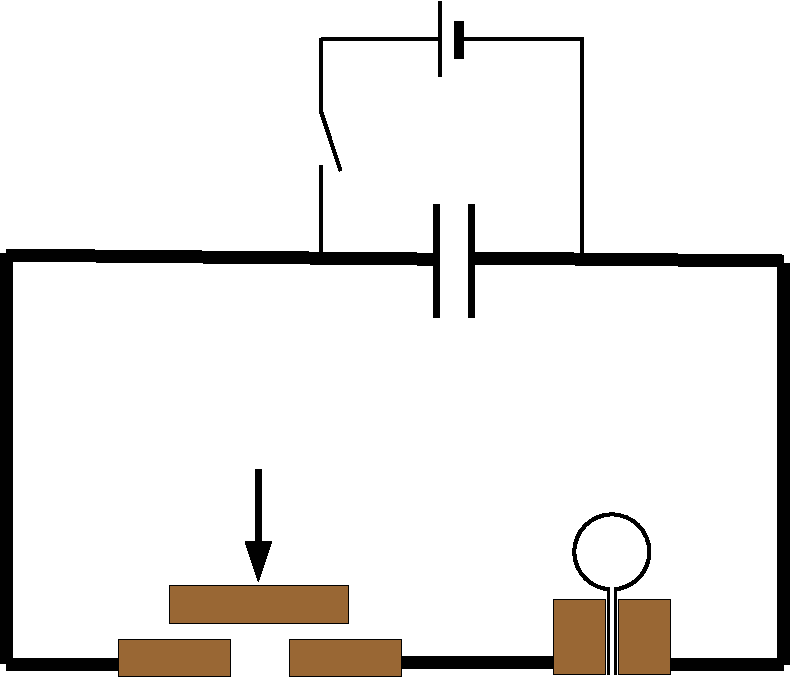
\includegraphics[width=0.9\textwidth]{images/circuit}
	\end{center}
\end{column}
\end{columns}

\end{frame}

\section{Meetmogelijkheden}
\subsection{Wijzigingen}
\begin{frame}
\begin{columns}
\begin{column}{0.5\textwidth}
	\begin{itemize}
	\item Oorspronkelijk
		\begin{itemize}
		\item $\derivs{B}{t}$ pickup-spoel
		\item[$\rightarrow$] Nieuw: 136\,mm$^2$
		\end{itemize}
	\item Onze toevoegingen
		\begin{itemize}
		\item Spanning over spoel
		\item Stroom (door shunt)
		\end{itemize}
	\end{itemize}
\end{column}
\begin{column}{0.5\textwidth}
	\begin{center}
	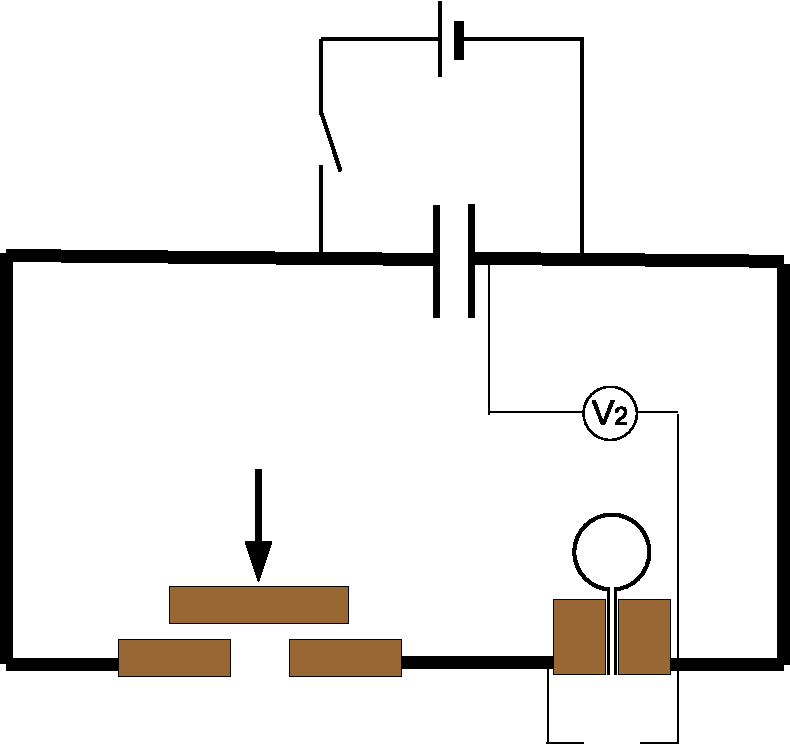
\includegraphics[width=0.9\textwidth]{images/circuit-new}
	\end{center}
\end{column}
\end{columns}
\end{frame}

\subsection{Calibratie}
\begin{frame}
\begin{center}
\includeGraph{0.85}{fitI800V}
\end{center}
\end{frame}

\begin{frame}
$$
\begin{array}{c|c|c|c}
V_0 (\mathrm V)&
	L (\mu\mathrm H)&
			R (\mathrm m \Omega)&
				\Rshunt (\mathrm m \Omega)\\\hline
71&	0.83 \pm 0.06&	12 \pm 3&	43 \pm 8\\
100&	0.84 \pm 0.03&	9 \pm 1&	9 \pm 1\\
200&	0.82 \pm 0.01&	8.3 \pm 0.6&	5.3 \pm 0.3\\
400&	0.82 \pm 0.01&	7.1 \pm 0.6&	2.0 \pm 0.1\\
800&	0.82 \pm 0.01&	7.7 \pm 0.7&	1.12 \pm 0.09\\
\end{array}
$$
\includeGraph{0.8}{RshuntPlot}
\end{frame}

\begin{frame}
\begin{columns}[c]
\begin{column}[c]{0.5\textwidth}
\includeGraph{0.7}{Ishunt}
\end{column}
\begin{column}[c]{0.5\textwidth}
\begin{center}
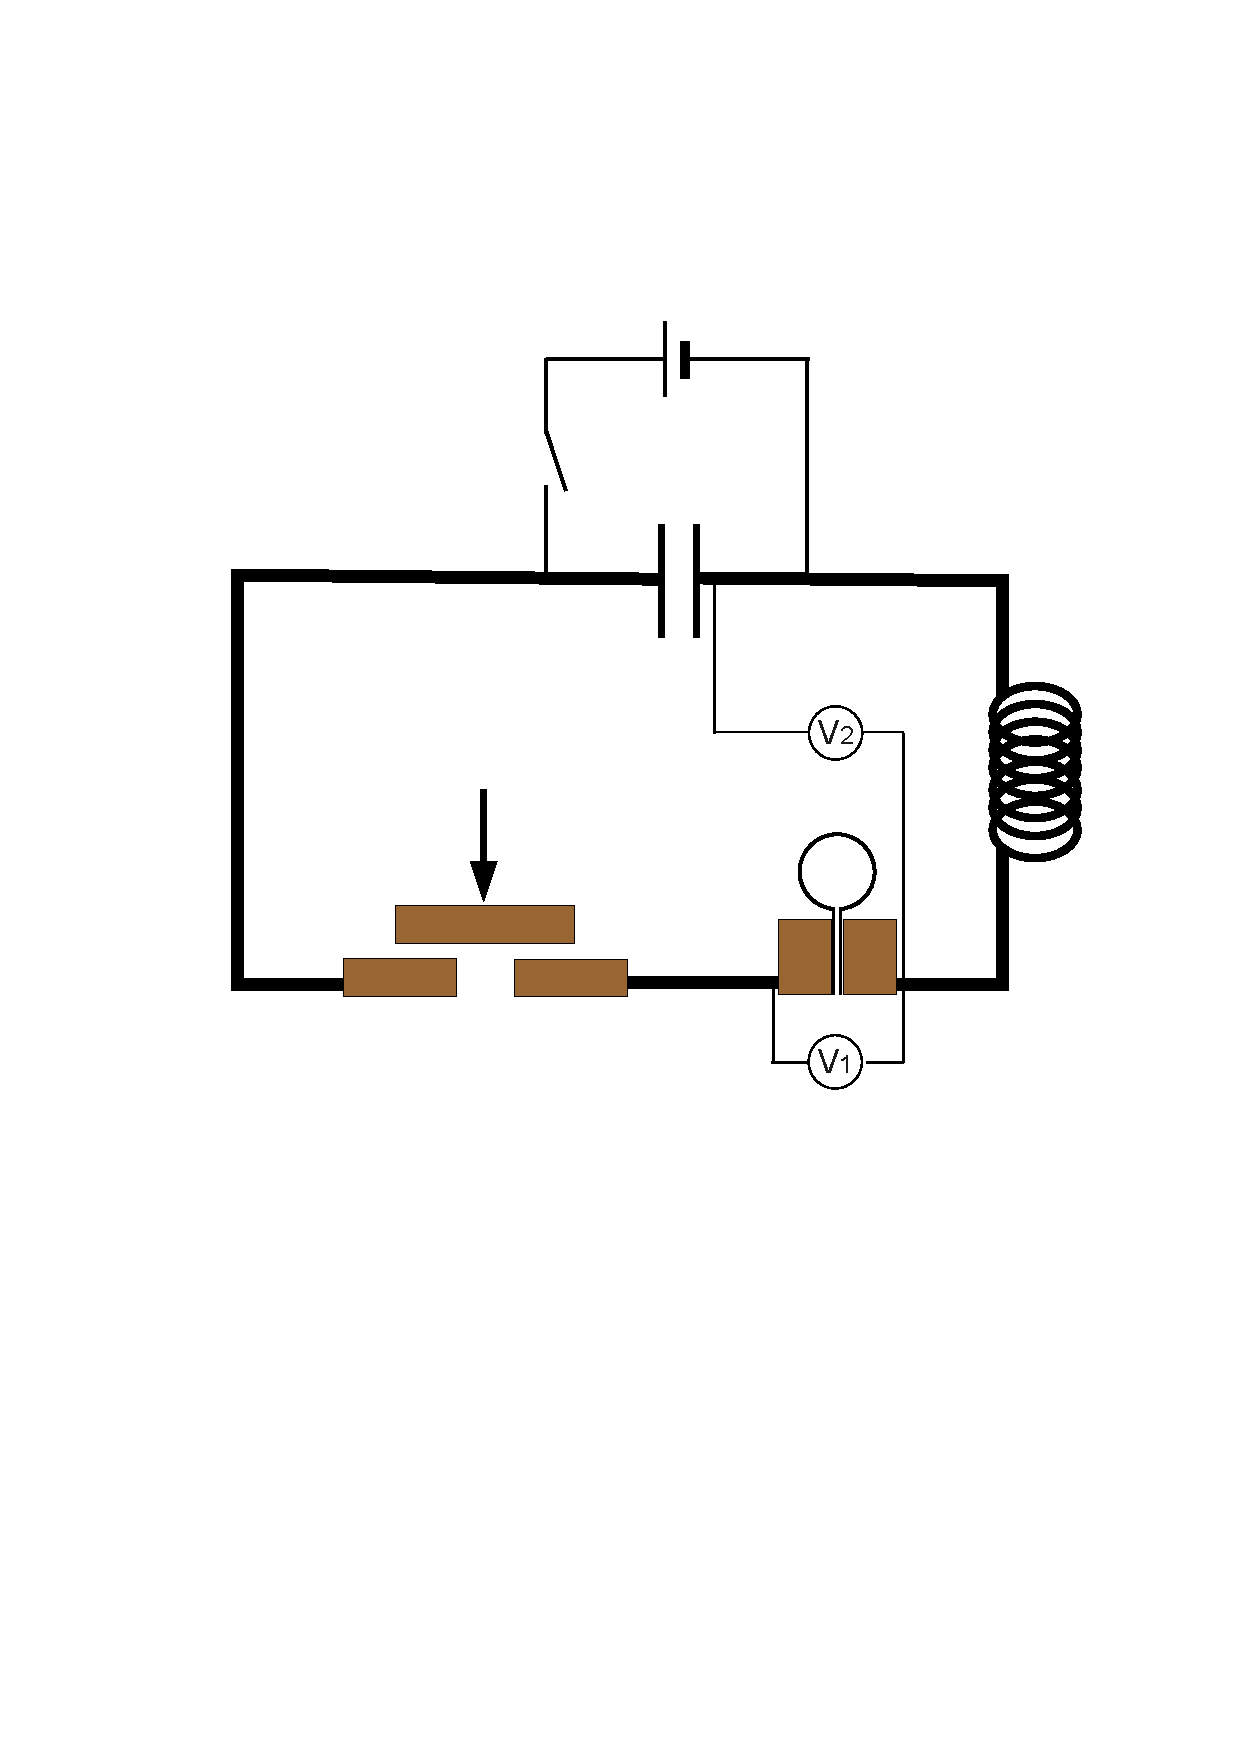
\includegraphics[width=1.0\textwidth]{images/circuit-new-inductance}
\end{center}
\end{column}
\end{columns}
\end{frame}

\end{document}
